\documentclass[12pt]{article}

\usepackage{sbc-template}
\usepackage{graphicx,url,booktabs}
\usepackage[utf8]{inputenc}
\usepackage[english]{babel}

\sloppy

\title{Statistical Analysis and Demand Prediction for Bike Sharing:\\
A DOE-Informed Observational Study}

\author{[First Author Name]\inst{1}, [Second Author Name]\inst{1}}

\address{[Department and University]\\
  Design of Experiments\\
  \email{[author emails]}
}

\begin{document}

\maketitle

\begin{abstract}
This study examines hourly bicycle rental demand using 17,379 observations from
the Capital Bikeshare system in Washington, D.C., collected in 2011 and 2012.
The data are observational and have a natural factorial and temporal structure.
We combine descriptive statistics, factorial analysis of variance, effect and
interaction plots, residual diagnostics, and two multiple regression models. The
central factorial result is the interaction between hour and working-day status,
with partial eta-squared 0.589. The interaction model for $\log(1+cnt)$ obtained
adjusted $R^2$ 0.927, although residual temporal dependence remained and
motivated HAC standard errors. A corresponding predictor was assessed with
expanding-window validation. On the final quarter of 2012, it obtained MAE
51.99, RMSE 83.07, and out-of-sample $R^2$ 0.830. The
results demonstrate strong temporal and weather associations, but the lack of
randomization prevents causal interpretation.
\end{abstract}

\begin{resumo}
Este estudo analisa a demanda horária por bicicletas usando 17.379 observações
do sistema Capital Bikeshare de Washington, D.C., coletadas em 2011 e 2012. Os
dados são observacionais e possuem estrutura fatorial natural e temporal. A
análise combina estatística descritiva, análise de variância fatorial, gráficos
de efeitos e interações, diagnóstico de resíduos e regressão múltipla. O
principal resultado fatorial é a interação entre hora e dia útil, com eta
quadrado parcial de 0,589. O modelo de interação para $\log(1+cnt)$ obteve
$R^2$ ajustado de 0,927, embora a dependência temporal residual tenha motivado
erros-padrão HAC. O preditor correspondente, avaliado com janelas temporais
expansivas, obteve MAE 51,99, RMSE 83,07 e $R^2$ fora da amostra de 0,830 no
último trimestre de 2012. A ausência de
randomização impede interpretações causais.
\end{resumo}

\section{Introduction}

Bike-sharing systems record demand at a high temporal resolution and provide a
useful view of urban mobility. Rental counts depend simultaneously on calendar,
seasonal, and meteorological conditions. This multi-factor structure makes the
data suitable for a Design of Experiments (DOE)-informed analysis, even though
the records were not produced by a controlled experiment.

The objective of this study is to identify and quantify factors and interactions
associated with hourly rental demand and to develop a predictor that generalizes
to later periods. The analysis emphasizes the interaction between hour and
working-day status: commuting should generate morning and evening peaks on
working days, while non-working days should show a smoother recreational
profile. We distinguish explanatory inference from predictive validation and
avoid causal language because no treatment was randomized.

\section{Dataset and Study Design}

The UCI Bike Sharing Dataset \cite{uci-bike-sharing} contains records from the
Capital Bikeshare system in Washington, D.C. The associated publication describes
the collection and its event-detection context \cite{fanaee2013}. We use the
hourly file, covering January 1, 2011 through December 31, 2012.

Each row is one observed hour. The response, \texttt{cnt}, is the total number
of rentals and equals \texttt{casual + registered}. Those components are not
used as predictors because they would cause direct target leakage. Factors
include hour, working-day status, weather category, season, and year. Temperature,
humidity, and wind speed are normalized continuous covariates. Apparent
temperature was omitted because its correlation with temperature was 0.988 and
their joint variance inflation factors exceeded 43.

The design is observational, unrandomized, unblocked, and naturally factorial.
It is neither a controlled factorial experiment nor an OFAT design. Observations
are ordered in time and therefore cannot be assumed independent. There are 165
missing timestamps in the complete hourly calendar sequence; no imputation was
performed because the models use observed hours rather than lagged responses.
Only three rows have weather level 4, so levels 3 and 4 were combined as
``precipitation/adverse'' for inferential stability while the original data were
kept unchanged.

\section{Methods}

\subsection{Descriptive and DOE-informed analyses}

We calculated sample sizes, means, medians, standard deviations, quartiles,
histograms, boxplots, temporal plots, and Pearson correlations. Main-effect plots
show group means with 95\% confidence intervals. The interaction plot focuses on
the prespecified hour by working-day relationship.

One-way ANOVA and median-centered Levene tests were calculated on the raw and
log-transformed responses. Factorial models were estimated with ordinary least
squares. Nested partial F tests evaluated the incremental contribution of
interaction, and a type-II ANOVA table reports partial eta-squared. Tukey HSD was
used only for descriptive weather contrasts. Because the design is observational
and unbalanced, inferential conclusions rely on effect magnitude and uncertainty,
not p-values alone \cite{montgomery2017}.

\subsection{Transformations and explanatory regression}

Raw \texttt{cnt}, $\sqrt{cnt}$, and $\log(1+cnt)$ were compared using Q--Q,
residual-versus-fitted, scale-location, Breusch--Pagan, Shapiro--Wilk (a fixed
5,000-residual subset), Jarque--Bera, and Durbin--Watson diagnostics. Box--Cox
maximum likelihood was also calculated \cite{boxcox1964}. The logarithmic scale
was retained for the MVP because it most reduced the Breusch--Pagan statistic,
improved adjusted $R^2$, and supports a multiplicative interpretation, although
none of the candidate scales fully satisfied classical assumptions.

Two hierarchical explanatory models were fitted. M0 contains the main effects of
hour, working-day status, weather, season, temperature, humidity, wind speed, and
year. M1 adds only the prespecified hour by working-day interaction and retains
both component main effects. This comparison directly tests whether the
factorial interaction adds information beyond an additive model. We compare
adjusted $R^2$, AIC, BIC, and a nested partial F test. Due to residual
autocorrelation, M1 coefficient uncertainty was also calculated with
Newey--West HAC covariance using 168 observed-hour lags \cite{neweywest1987}.

\subsection{Chronological predictive validation}

Predictive evaluation was separate from full-sample inference. Models were
trained through March 2012 and evaluated on Q2, then trained through June and
evaluated on Q3. Mean RMSE across these two expanding-window validation periods
selected the specification. Q4 2012 was untouched until selection and served as
the final holdout. This avoids the temporal leakage caused by random splitting.

The predictive models used a continuous time index instead of a categorical year
effect. We compared an additive model (P0), the hour by working-day model (P1),
and a historical-mean baseline for each hour by working-day combination. Count
predictions from the log scale used Duan's smearing correction \cite{duan1983}.
We report MAE, RMSE, RMSLE, and out-of-sample $R^2$.

\section{Results}

\subsection{Descriptive results}

Table~\ref{tab:descriptive} summarizes the response. Its mean exceeds its median,
and the raw distribution is right-skewed (skewness 1.277).

\begin{table}[ht]
\centering
\caption{Descriptive statistics for hourly total rentals.}
\label{tab:descriptive}
\resizebox{\columnwidth}{!}{\begin{tabular}{rrrrrrrr}
\toprule
N & Mean & Median & SD & Q1 & Q3 & Min & Max \\
\midrule
17379 & 189.463 & 142.000 & 181.388 & 40.000 & 281.000 & 1.000 & 977.000 \\
\bottomrule
\end{tabular}
}
\end{table}

Mean hourly demand was 204.87 under clear/partly cloudy weather, 175.17 under
mist/cloudy weather, and 111.50 under precipitation/adverse weather. Seasonal
means were 111.11 in spring, 208.34 in summer, 236.02 in fall, and 198.87 in
winter. These are unadjusted associations and reflect imbalances among other
conditions.

\begin{figure}[ht]
\centering
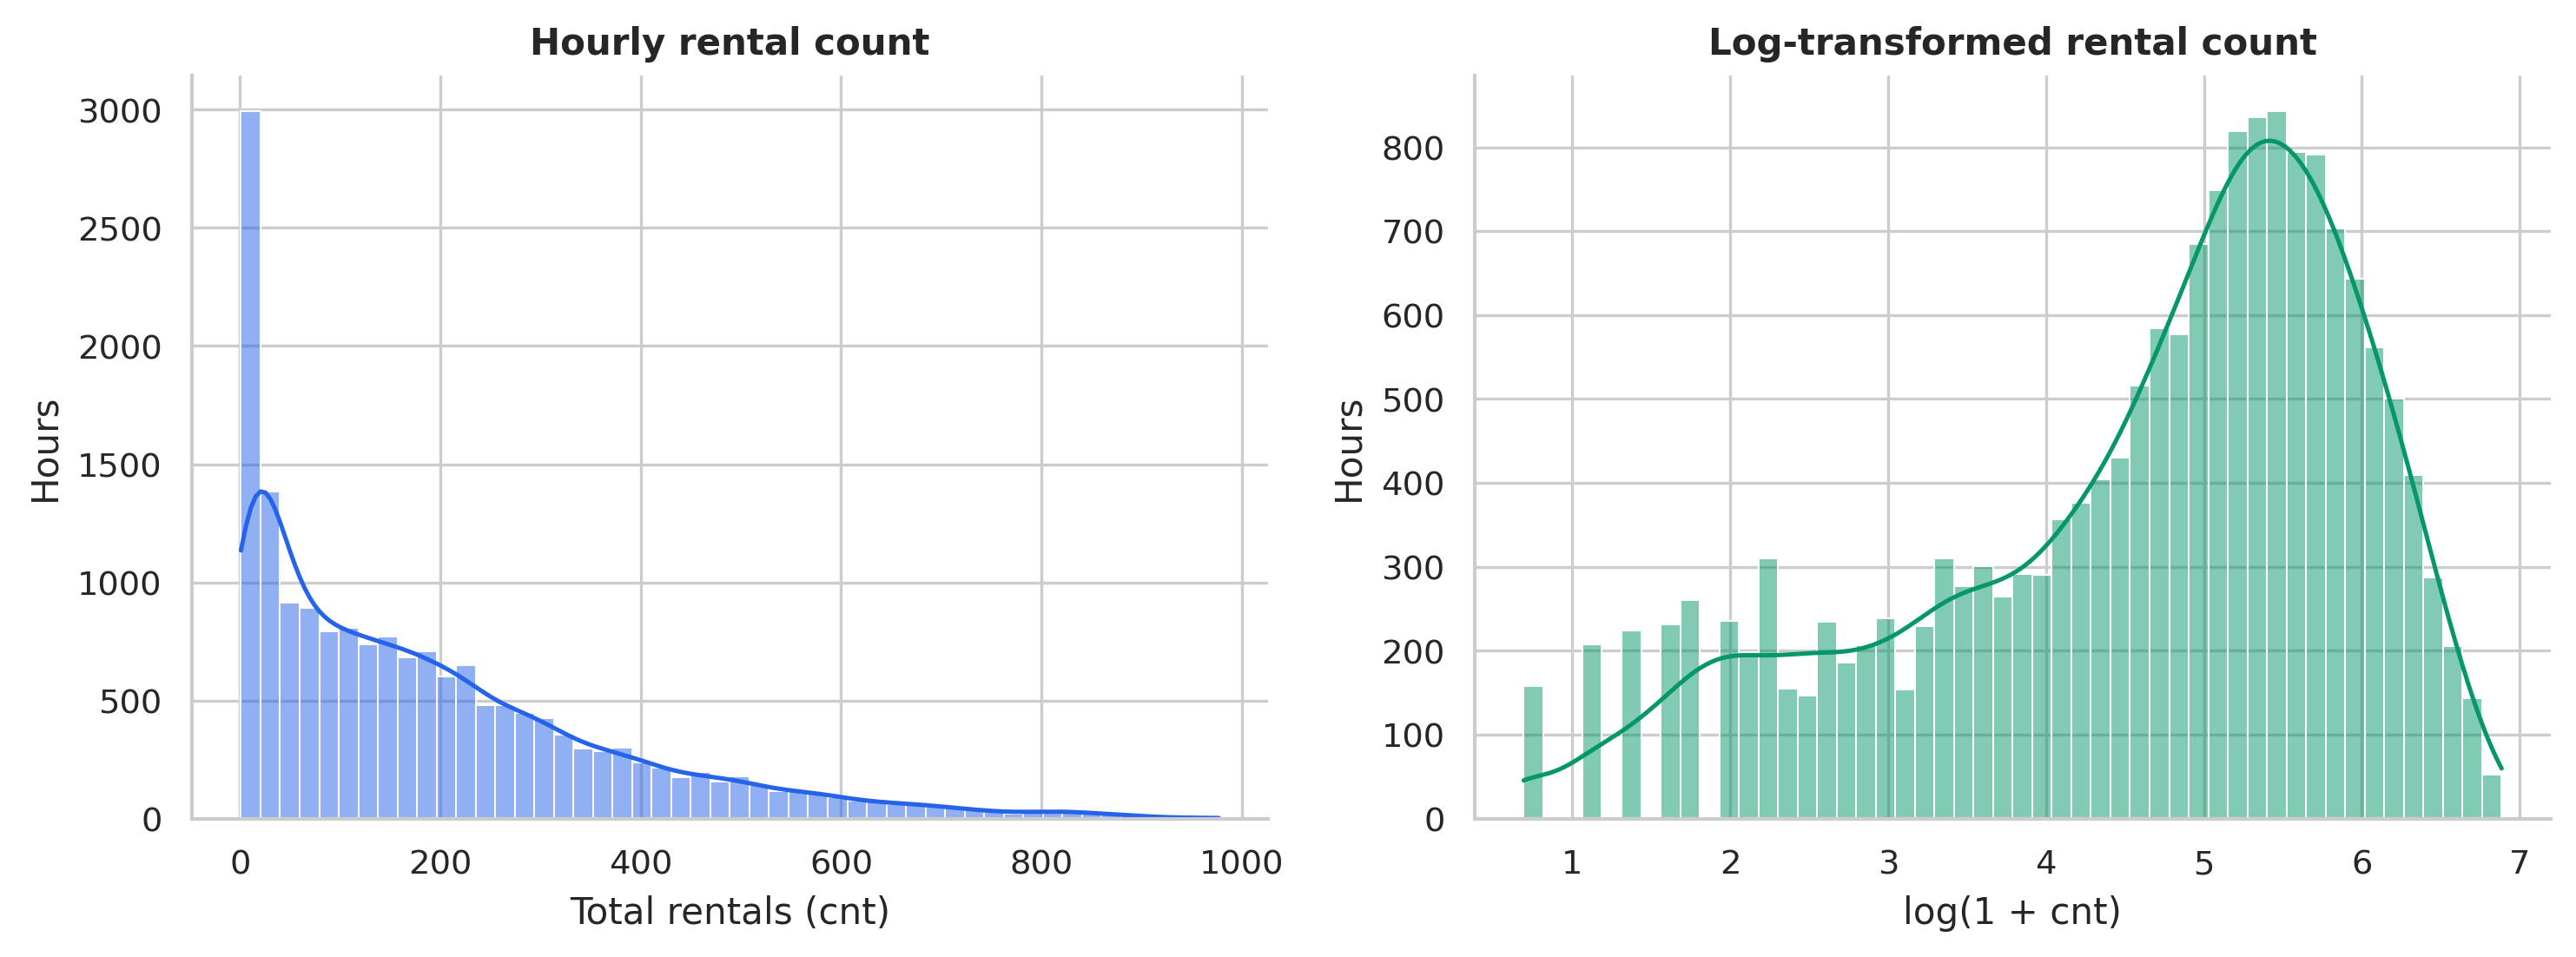
\includegraphics[width=\columnwidth]{../outputs/figures/response_distributions.png}
\caption{Raw and log-transformed hourly rental distributions.}
\label{fig:distribution}
\end{figure}

\subsection{Main effects and interactions}

Figure~\ref{fig:interactions} shows the central result. On working days, demand
peaks near 08:00 and 17:00--18:00. Non-working days show a broader midday peak.
Consequently, the small adjusted main effect of working-day status must not be
interpreted without hour.

\begin{figure}[ht]
\centering
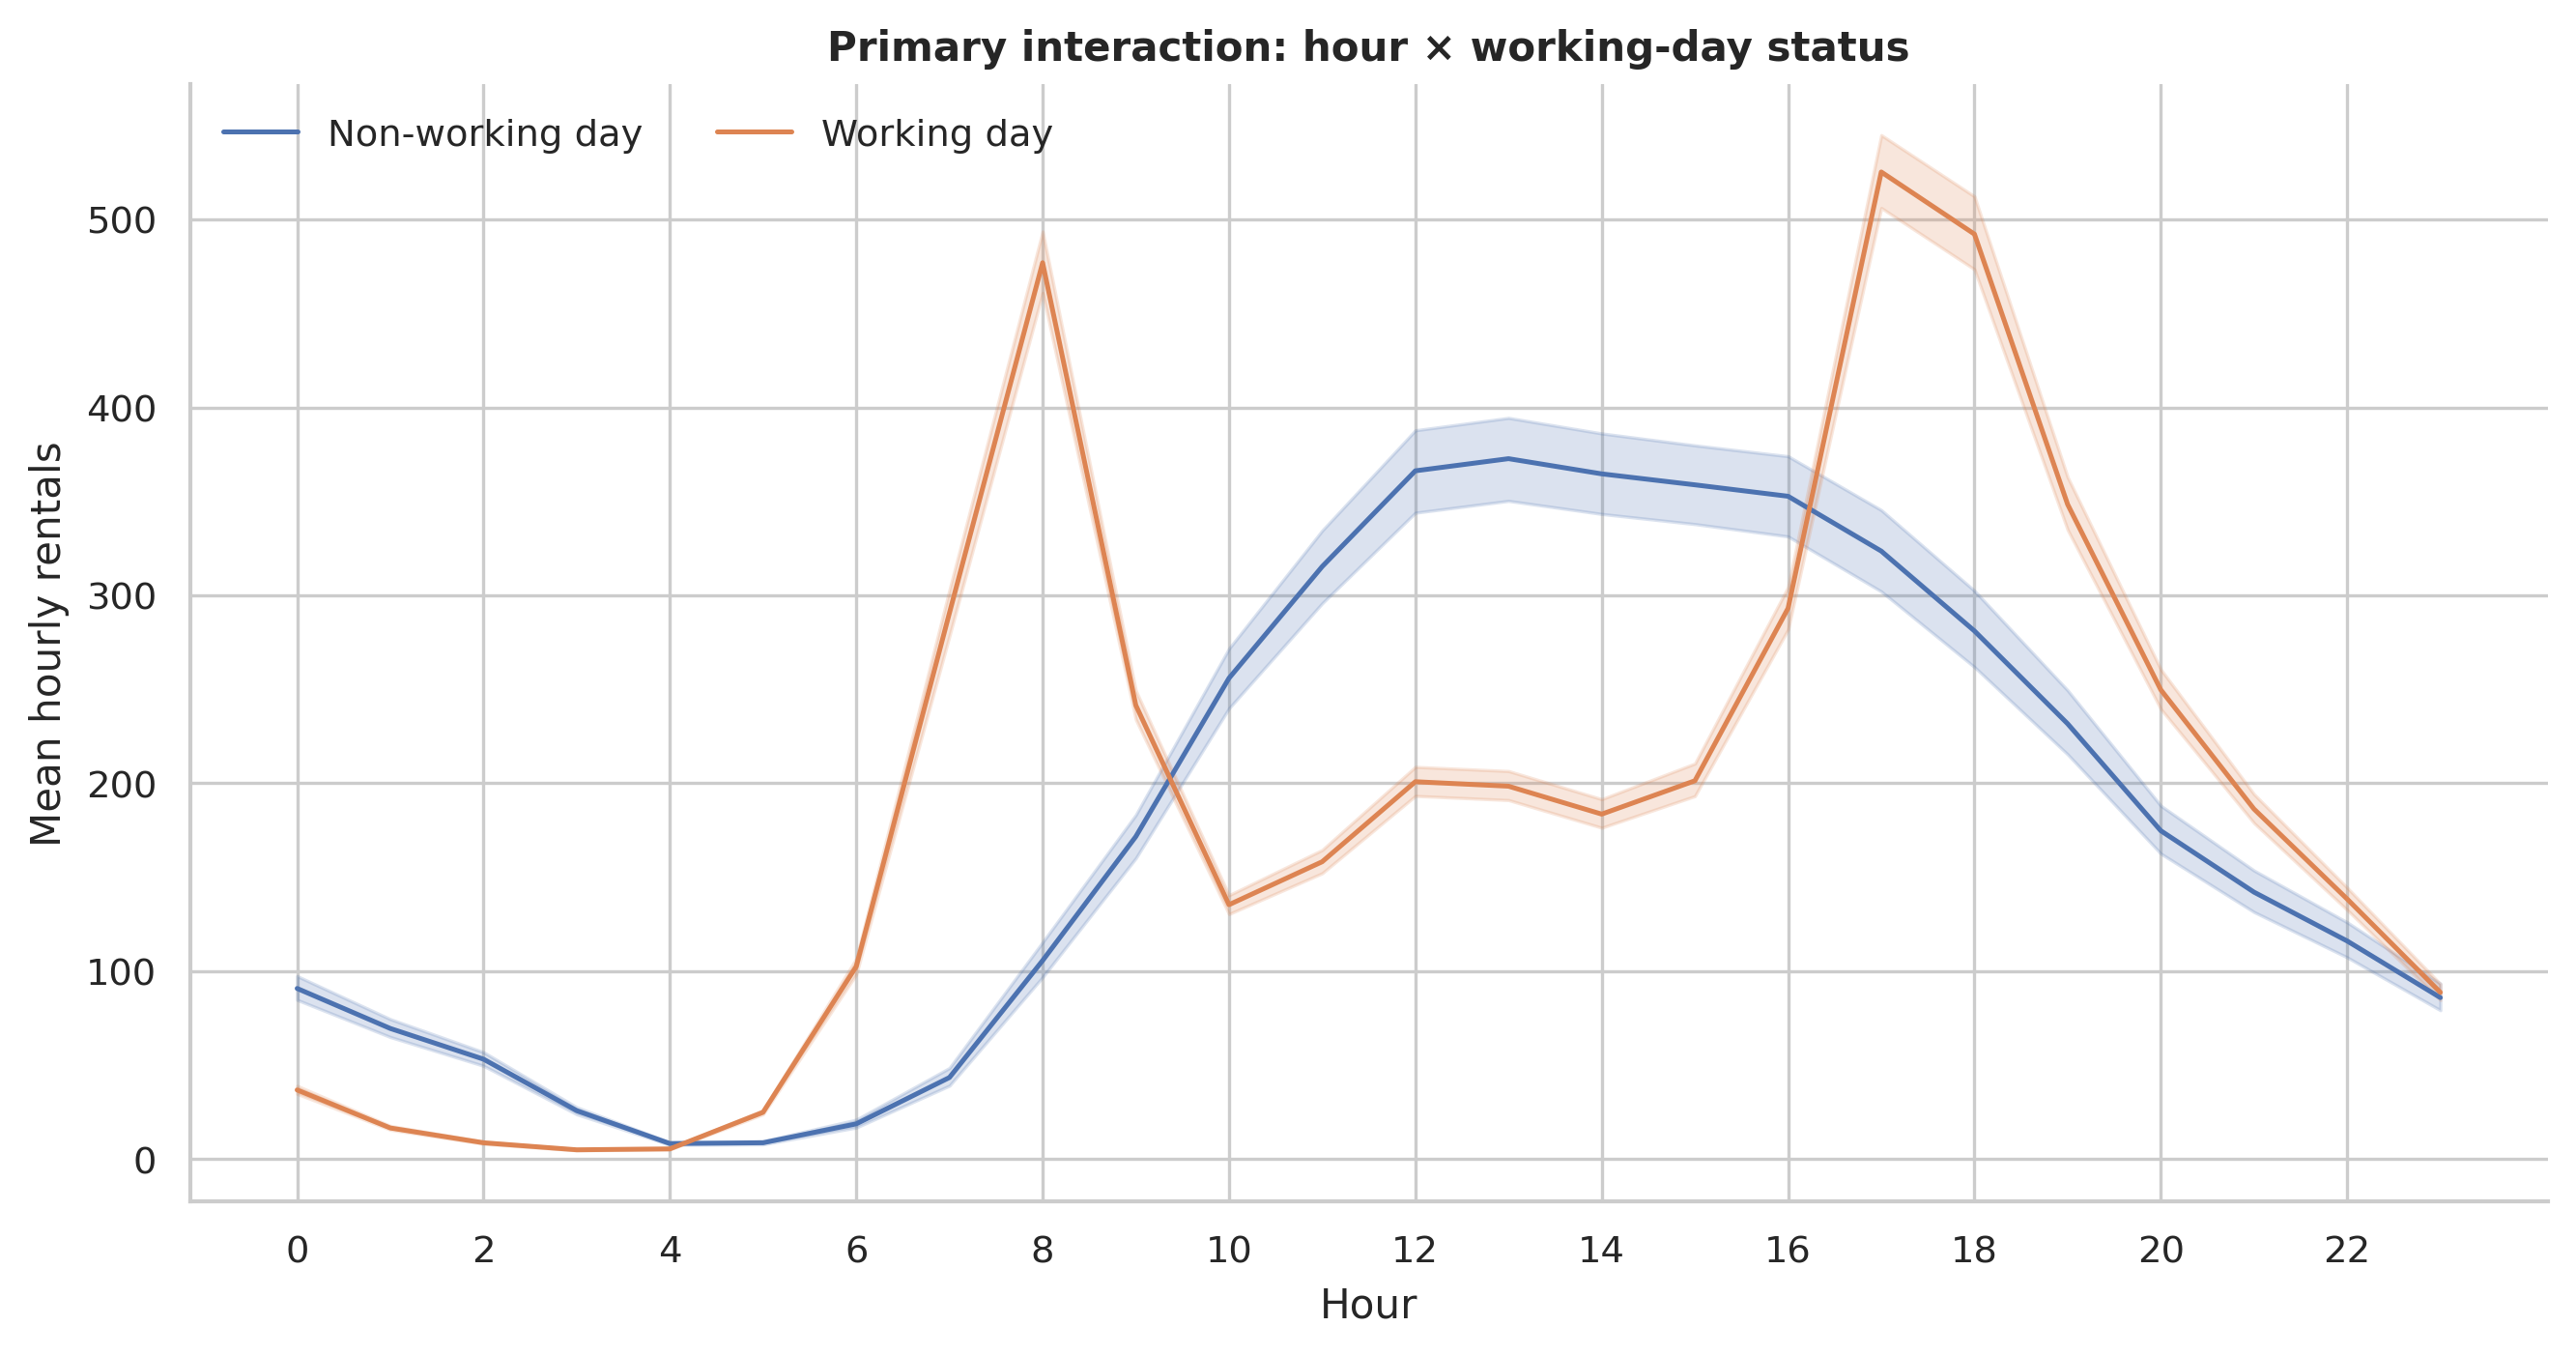
\includegraphics[width=\columnwidth]{../outputs/figures/primary_interaction.png}
\caption{The primary observed interaction between hour and working-day status.}
\label{fig:interactions}
\end{figure}

M1's partial eta-squared was 0.878 for hour and 0.589 for hour by working day
(Table~\ref{tab:anova}). Year had partial eta-squared 0.264, reflecting higher
adoption in 2012. Weather and season also showed meaningful adjusted
associations, with partial eta-squared 0.120 and 0.168. All three descriptive
weather Tukey contrasts on $\log(1+cnt)$ rejected equality ($p<0.001$).

\begin{table}[ht]
\centering
\caption{Type-II ANOVA for the M1 interaction model.}
\label{tab:anova}
\resizebox{\columnwidth}{!}{\begin{tabular}{lrrlr}
\toprule
Term & df & F & p-value & Partial eta-squared \\
\midrule
Hour & 23.000 & 6050.916 & $<0.001$ & 0.890 \\
Working day & 1.000 & 19.488 & $<0.001$ & 0.001 \\
Weather & 2.000 & 1283.947 & $<0.001$ & 0.130 \\
Season & 3.000 & 820.348 & $<0.001$ & 0.125 \\
Year & 1.000 & 6367.468 & $<0.001$ & 0.270 \\
Hour x working day & 23.000 & 1195.618 & $<0.001$ & 0.615 \\
Weather x hour & 46.000 & 7.820 & $<0.001$ & 0.020 \\
Season x hour & 69.000 & 8.444 & $<0.001$ & 0.033 \\
Temperature & 1.000 & 2253.208 & $<0.001$ & 0.116 \\
Temperature squared & 1.000 & 1020.639 & $<0.001$ & 0.056 \\
Humidity & 1.000 & 287.999 & $<0.001$ & 0.016 \\
Wind speed & 1.000 & 198.396 & $<0.001$ & 0.011 \\
\bottomrule
\end{tabular}
}
\end{table}

\subsection{Model diagnostics and explanatory fit}

The Box--Cox estimate was 0.305. For M1, adjusted $R^2$ rose from 0.812 on the
raw response to 0.893 on the square-root scale and 0.927 on the log scale. The
Breusch--Pagan statistic fell from 4282.8 to 2039.7 and 1672.5, respectively, but
all associated p-values remained below 0.001. The log-scale Durbin--Watson
statistic was 0.775 in M1. Residual ACF was 0.612 at lag 1,
0.243 at lag 24, and 0.200 at lag 168. Thus, the model is informative but its
classical independence assumption is violated.

Adding hour by working day produced a large improvement, raising adjusted
$R^2$ from 0.824 to 0.927 and reducing BIC from 31587.2 to 16356.7
(Table~\ref{tab:models}). The nested test also supported the interaction
($F=1079.55$, $p<0.001$). M1 uses 57 parameters because a 24-level hour factor
interacts with a binary factor; the paper interprets the interaction curve rather
than listing every dummy coefficient.

\begin{table}[ht]
\centering
\caption{Simple explanatory comparison on $\log(1+cnt)$.}
\label{tab:models}
\resizebox{\columnwidth}{!}{\begin{tabular}{lrrrr}
\toprule
Model & Parameters & Adjusted R-squared & AIC & BIC \\
\midrule
M0 & 34 & 0.824 & 31323.298 & 31587.241 \\
M1 & 57 & 0.927 & 15914.181 & 16356.673 \\
M2 & 103 & 0.929 & 15681.777 & 16481.368 \\
M3 & 172 & 0.931 & 15187.880 & 16523.119 \\
M4 & 173 & 0.935 & 14188.397 & 15531.399 \\
\bottomrule
\end{tabular}
}
\end{table}

\subsection{Predictive performance}

P1, which includes hour by working day, had the lowest mean validation RMSE
(135.77) across Q2 and Q3 2012. The additive P0 obtained 171.30, and the baseline
obtained 167.14. The comparison shows that the same interaction emphasized by
the DOE analysis also improves prediction.

On the Q4 holdout, P1 obtained MAE 51.99, RMSE 83.07, $R^2=0.830$, and RMSLE
0.524 (Table~\ref{tab:holdout}). The hour-by-working-day baseline obtained RMSE
119.59 and $R^2=0.648$. P1 errors were largest around 17:00--18:00, when demand
was also highest.

\begin{table}[ht]
\centering
\caption{Performance on the untouched Q4 2012 holdout.}
\label{tab:holdout}
\resizebox{\columnwidth}{!}{\begin{tabular}{lrrrr}
\toprule
Model & MAE & RMSE & R-squared & RMSLE \\
\midrule
Baseline & 79.950 & 119.589 & 0.648 & 0.604 \\
P0 & 84.224 & 120.924 & 0.640 & 0.703 \\
P1 & 50.176 & 81.651 & 0.836 & 0.501 \\
P2 & 50.749 & 82.509 & 0.832 & 0.498 \\
\bottomrule
\end{tabular}
}
\end{table}

\begin{figure}[ht]
\centering
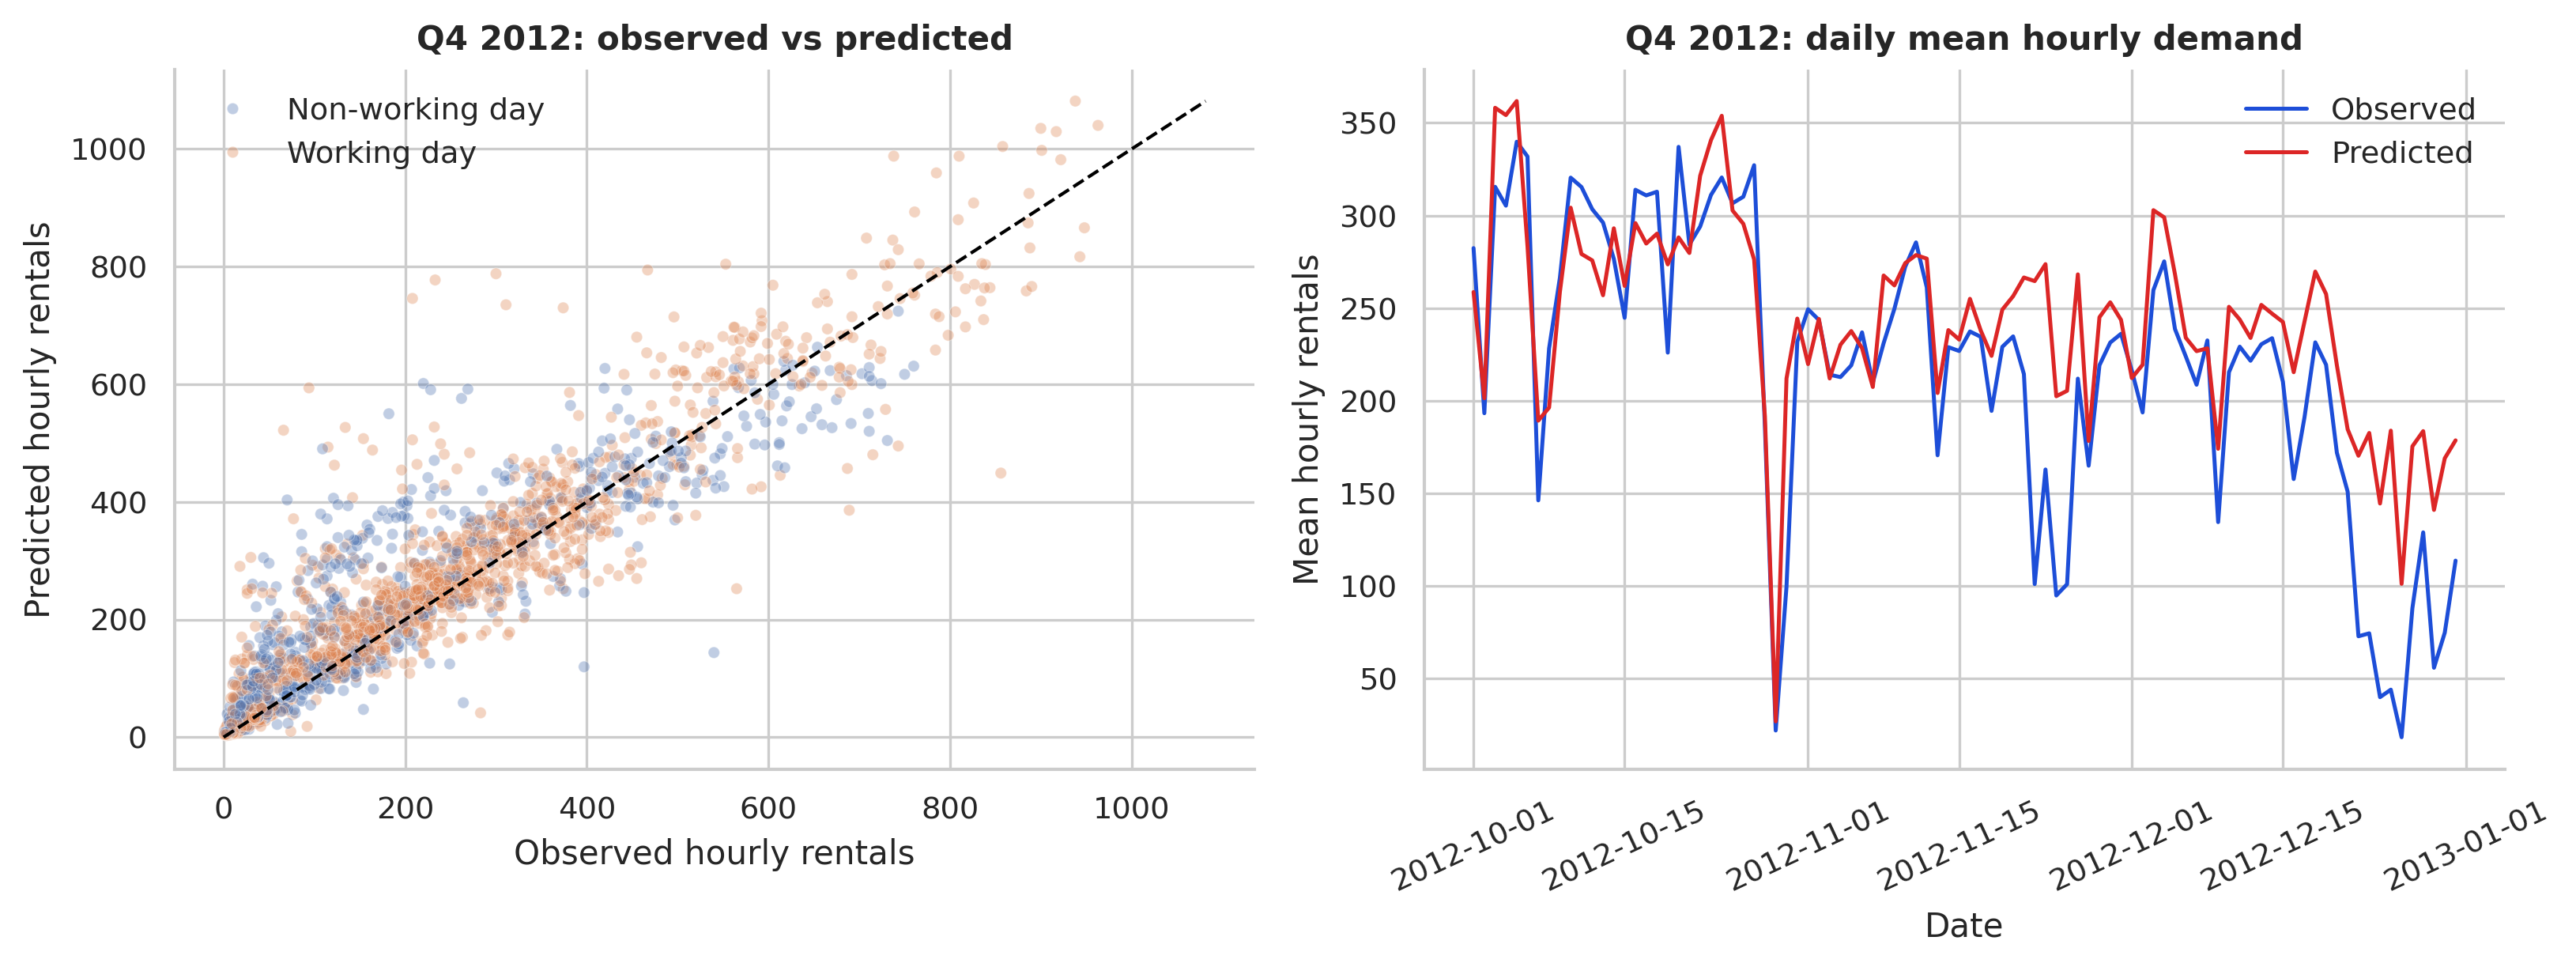
\includegraphics[width=\columnwidth]{../outputs/figures/holdout_predictions.png}
\caption{Final holdout predictions from the selected P1 model.}
\label{fig:predictions}
\end{figure}

\section{Discussion and Limitations}

Hour is the dominant observed factor, but its meaning depends strongly on
working-day status. This validates the factorial approach: an OFAT analysis of
working days would obscure the commuting profile. Weather, season, temperature,
humidity, wind, and year provide adjustment, while one interaction remains the
clear focus of the narrative.

The analysis has important limitations. Treatments were not randomized, so
unmeasured events, system expansion, and temporal trends may confound estimates.
Residual autocorrelation remains after the included factors, and HAC correction
changes uncertainty rather than the fitted mean. The Q4 holdout measures one
future season rather than all possible deployment conditions. The three severe
weather records cannot support a separate stable estimate. Finally, this
simplified analysis does not compare mixed-effects, autoregressive, nonlinear,
or negative-binomial models.

\section{Conclusion}

The DOE-informed analysis identified the hour by working-day interaction as the
main structural feature of hourly bicycle demand. Adding this single interaction
raised adjusted $R^2$ from 0.824 to 0.927. The corresponding predictor explained
83.0\% of count variation in the final temporal holdout. The deliberately narrow
M0--M1 comparison demonstrates the value of factorial reasoning without relying
on a large collection of exploratory models. Before submission, we will compile
and visually review the paper in the SBC environment and replace author
placeholders.

\bibliographystyle{sbc}
\bibliography{references}

\end{document}
